\let\negmedspace\undefined
\let\negthickspace\undefined
\documentclass[journal]{IEEEtran}
\usepackage[a5paper, margin=10mm, onecolumn]{geometry}
%\usepackage{lmodern} % Ensure lmodern is loaded for pdflatex
\usepackage{tfrupee} % Include tfrupee package

\setlength{\headheight}{1cm} % Set the height of the header box
\setlength{\headsep}{0mm}     % Set the distance between the header box and the top of the text

\usepackage{gvv-book}
\usepackage{gvv}
\usepackage{cite}
\usepackage{amsmath,amssymb,amsfonts,amsthm}
\usepackage{algorithmic}
\usepackage{graphicx}
\usepackage{textcomp}
\usepackage{xcolor}
\usepackage{txfonts}
\usepackage{listings}
\usepackage{enumitem}
\usepackage{mathtools}
\usepackage{gensymb}
\usepackage{comment}
\usepackage[breaklinks=true]{hyperref}
\usepackage{tkz-euclide} 
\usepackage{listings}
% \usepackage{gvv}                                        
\def\inputGnumericTable{}                                 
\usepackage[latin1]{inputenc}                                
\usepackage{color}                                            
\usepackage{array}                                            
\usepackage{longtable}                                       
\usepackage{calc}                                             
\usepackage{multirow}                                         
\usepackage{hhline}                                           
\usepackage{ifthen}                                           
\usepackage{lscape}
\begin{document}

\bibliographystyle{IEEEtran}
\vspace{3cm}



\title{11.16.2.2.1}
\author{EE24BTECH11020 - Ellanti Rohith}
{\let\newpage\relax\maketitle}
\textbf{Question:} A die is thrown. Find the probability of following event: The outcome is less than 7.
\\
\textbf{Solution:}The sample space for a fair six-sided die is:
\[
S = \{1,2,3,4,5,6\}
\]
\begin{center}
\begin{tabular}{|c|c|c|}
\hline 
\textbf{Variable name} & \textbf{Description} \\
\hline 
$\vec{S}$ & Sample space \\
\hline 
$\vec{X}$ & Random variable corresponding to the number on die \\
\hline

$F_{\vec{X}} (x)$ & Cumulative distribution function ( CDF ) \\
\hline
$p_{\vec{X}} (x)$ & Probability Mass function ( PMF ) \\
\hline
\end{tabular}
\end{center}
Each outcome is equally likely.

Let \( X \) be the number obtained when the die is rolled.

\[
X \in S
\]
\begin{tabular}{|l|c l|c l|}
    \hline
    & (a) & & (b) & \\
    \hline
    Postulate 2 & $A + 0 = A$ & & $A \cdot 1 = A$ & \\
    \hline
    Postulate 5 & $A + A' = 1$ & & $A
    \cdot A' = 0$ & \\
    \hline
    Theorem 1 & $A + A = A$ & & $A \cdot A = A$ & \\
    \hline
    Theorem 2 & $A + 1 = 1$ & & $A \cdot 0 = 0$ & \\
    \hline
    Theorem 3, involution & $(A')' = A$ & & - & \\
    \hline
    Postulate 3, commutative & $A + B = B + A$ & & $AB = BA$ & \\
    \hline
    Theorem 4, associative & $A + (B + C) = (A + B) + C$ & & $A(BC) = (AB)C$ & \\
    \hline
    Postulate 4, distributive & $A(B + C) = AB + AC$ & & $A + BC = (A + B)(A + C)$ & \\
    \hline
    Theorem 5, DeMorgan & $(A + B)' = A' B'$ & & $(AB)' = A' + B'$ & \\
    \hline
    Theorem 6, absorption & $A + AB = A$ & & $A(A + B) = A$ & \\
    \hline
\end{tabular}


Since the die is fair, each outcome has an equal probability:

\[
p_X(k) =
\begin{cases}
\frac{1}{6}, & k \in \{1,2,3,4,5,6\} \\
0, & \text{otherwise}
\end{cases}
\]

By the definition of the cumulative distribution function (CDF):

\[
F_X(k) = P(X \leq k) = \sum_{i=-\infty}^{k} p_X(i)
\]

Thus, the CDF is given by:

\[
F_X(k) =
\begin{cases}
0, & k < 1 \\
\frac{1}{6}, & 1 \leq k < 2 \\
\frac{2}{6}, & 2 \leq k < 3 \\
\frac{3}{6}, & 3 \leq k < 4 \\
\frac{4}{6}, & 4 \leq k < 5 \\
\frac{5}{6}, & 5 \leq k < 6 \\
1, & k \geq 6
\end{cases}
\]
We need to find:
\[
P(X < 7) = P(X \leq 6) = \sum_{i=1}^{6} P(X = i)\\
= \frac{1}{6} + \frac{1}{6} + \frac{1}{6} + \frac{1}{6} + \frac{1}{6} + \frac{1}{6}
\]

\[
= \frac{6}{6} = 1
\]

Thus,
\[
P(X < 7) = 1
\]

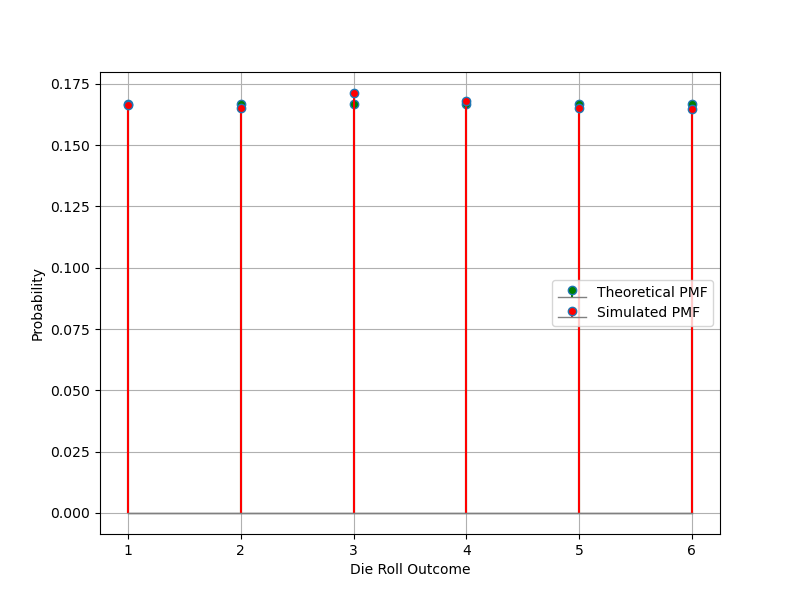
\includegraphics[width=\textwidth]{Figs/Figure_1.png}
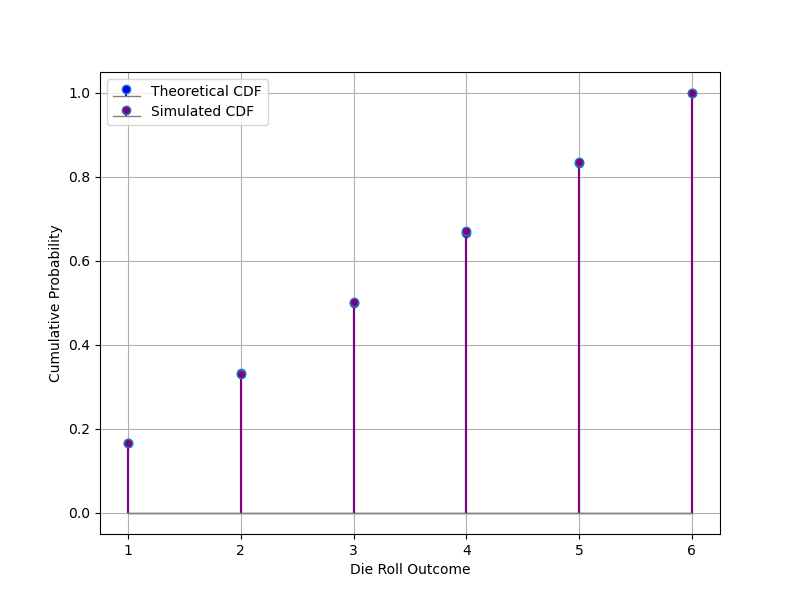
\includegraphics[width=\textwidth]{Figs/Figure_2.png}
\end{document}
